% Gerado por scripts/gerar-figuras-monografia.py; não editar.
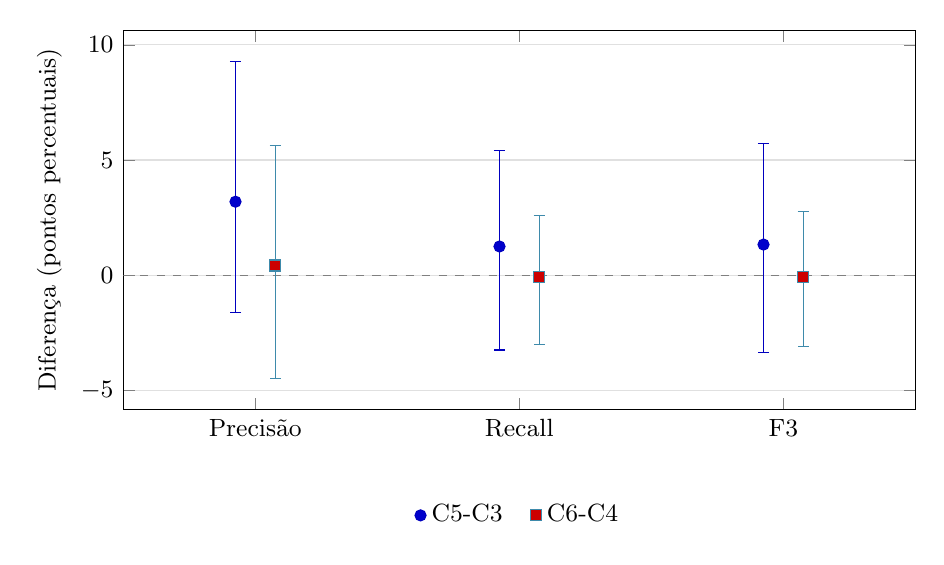
\begin{tikzpicture}
\begin{axis}[
width=0.96\textwidth,height=6.4cm,
tick label style={font=\small},label style={font=\small},
legend style={font=\small,at={(0.5,-0.22)},anchor=north,legend columns=3,draw=none,/tikz/every even column/.append style={column sep=8pt}},
ymajorgrids=true,grid style={black!12},
xmin=0.5,xmax=3.5,ylabel={Diferença (pontos percentuais)},xtick={1,2,3},xticklabels={Precisão,Recall,F3}
]
\addplot[black!50,dashed,forget plot] coordinates {(0.5,0) (3.5,0)};
\addplot+[only marks,color=blue!75!black,error bars/.cd,y dir=both,y explicit] coordinates {(0.92500000,3.18843898) += (0,6.07279336) -= (0,4.80556317) (1.92500000,1.24342420) += (0,4.18475529) -= (0,4.49905567) (2.92500000,1.32707387) += (0,4.37150277) -= (0,4.68422681)};
\addlegendentry{C5-C3}
\addplot+[only marks,color=cyan!65!black,error bars/.cd,y dir=both,y explicit] coordinates {(1.07500000,0.41788669) += (0,5.22151223) -= (0,4.89168737) (2.07500000,-0.09564802) += (0,2.70297448) -= (0,2.91229883) (3.07500000,-0.08985398) += (0,2.84265537) -= (0,3.02768540)};
\addlegendentry{C6-C4}
\end{axis}
\end{tikzpicture}
